\documentclass[letterpaper,12pt]{article}
\usepackage{epsfig,latexsym,amsmath,amssymb,epic,eepic,psfrag,subfigure,float,euscript,array}
\usepackage[latin1]{inputenc}
\usepackage{tikz,pgf,pgfplots}
\usepackage[margin=2.5cm]{geometry}
\usepackage[amssymb]{SIunits}
\usepackage{url}
\newenvironment{exercise}[1][Uppgift]{\begin{trivlist} \item[\hskip
    \labelsep {\stepcounter{exerctr}\bfseries #1
      \arabic{exerctr}}]}{\end{trivlist}\vspace{10mm}}

\newcounter{exerctr}
\newcounter{abcctr}[exerctr]

\newcommand{\abc}{\noindent\vspace{1mm}\\ {\bf
    \stepcounter{abcctr}(\alph{abcctr})\ }}
\newcommand{\bbm}{\begin{bmatrix}}
\newcommand{\ebm}{\end{bmatrix}}
\newcommand{\point}[1]{\hfill {\bf (#1p)}\\ \vspace{-5mm}}
\newcommand{\ctrb}{\EuScript{S}}
\newcommand{\Lap}{\mathcal{L}}
\newcommand{\obsv}{\EuScript{O}}
\newcommand{\realdel}[1]{\text{Re}\left\{#1\right\}}
\newcommand{\imagdel}{\text{Im}}
\newcommand{\bC}{\mathbb{C}}
\newcommand{\bR}{\mathbb{R}}
\newcommand{\bmpv}{\begin{minipage}[t]}
\newcommand{\bmps}{\begin{minipage}[t]{45mm}}
\newcommand{\bmpm}{\begin{minipage}[t]{90mm}}
\newcommand{\bmpl}{\begin{minipage}[t]{\textwidth}}
\newcommand{\emp}{\end{minipage}}
\newcommand*{\zethree}{\big(z - \mexp{-3h}\big)}
\newcommand*{\mexp}[1]{\ensuremath{\mathrm{e}^{#1}}}

\newcommand*\circled[1]{\tikz[baseline=(char.base)]{
            \node[shape=circle,draw,inner sep=2pt] (char) {#1};}}

\addtolength{\topmargin}{-1cm}
\textheight 23.5cm
%\oddsidemargin 0.61cm
%\evensidemargin 0.61cm



\title{Control Computarizado final exam (29\%)}
\author{Kjartan Halvorsen}

\begin{document}

\maketitle


\begin{description}
\item[Time] 2017-11-13 07:00 - 2017-11-14 17:30
\item[Permitted aids] Whatever books, notes, web pages, videos you can find. \textbf{Except} help from another living person. For questions about the exam I can be contacted at \url{kjartan@itesm.mx} or if acute by WhatsApp (556219 4048).
\end{description}

All answers should be readable and well motivated (if nothing else is written). Hand in (on paper) at the time of the class Tuesday November 14 at 17:30.

\begin{center}
{\Large Good luck!} \\
\end{center}


%-----------------------------------------------------------------

\subsubsection*{An inverted pendulum}

\noindent
\begin{minipage}{0.6\linewidth}
The cart-pendulum system is a common example of an unstable system. If we are not concerned with the position of the cart, but only with the angle of the pendulum, then the system can be simplified and written as 
\begin{align}
\frac{d}{dt} \bbm \theta\\\dot{\theta} \ebm &= \bbm \dot{\theta}\\\frac{mgl}{J} \sin\theta + \frac{1}{J}\cos\theta u \ebm, \qquad y = \theta,
 \end{align}
where $J$ is the moment of inertia of the pendulum. 
\end{minipage}
\begin{minipage}{0.3\linewidth}
\begin{center}
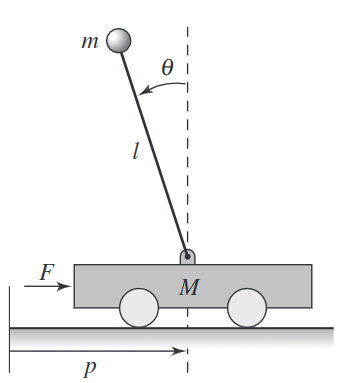
\includegraphics[width=\linewidth]{cart-pendulum.png}\\
{\tiny From the textbook}
\end{center}
\end{minipage}

\subsection*{Problem 1}
%-----------------------------
% Discretization
%-----------------------------

\subsubsection*{(a)}
Show that linearizing the model about the vertical equilibrium state ($\sin\theta \approx \theta$, $\cos\theta \approx 1$) gives the linear state-space system
\begin{equation}
\begin{aligned}
\frac{d}{dt}  \bbm \theta\\\dot{\theta} \ebm &= \bbm 0 & 1\\ \frac{mgl}{J} & 0\ebm \bbm \theta\\\dot{\theta} \ebm + \bbm 0\\\frac{1}{J} \ebm u\\
y &= \bbm 1 & 0 \ebm \bbm \theta\\\dot{\theta} \ebm.
\end{aligned}
\label{eq:sscont}
\end{equation}

\subsubsection*{(b)}
Show that the linear state space model corresponds to the transfer function 
\begin{equation}
G(s) = C \big( sI- A\big)^{-1} B = \frac{ 1/J }{s^2 - \frac{mgl}{J}},
\end{equation}
with poles in \(\pm \omega_0\) where \(\omega_0 = \sqrt{\frac{mgl}{J}}\).


\subsubsection*{(c)}
Here, and in the rest of the exam let $J=1$. Show that the zero-order-hold discretization of the state space model \eqref{eq:sscont} gives the discrete-time state space model
\begin{equation}
\begin{aligned}
x(kh+h) &= \underbrace{\bbm \cosh(\omega_0h) & \frac{1}{\omega_0}\sinh(\omega_0h)\\
                            \omega_0\sinh(\omega_0h) & \cosh(\omega_0h) \ebm}_{\Phi} x(kh) 
       + \underbrace{\bbm \frac{1}{\omega_0^2}(\cosh(\omega_0h)-1)\\ \
                               \frac{1}{\omega_0}\sinh(\omega_0h) \ebm}_{\Gamma} u(kh)\\
y(kh) &= \underbrace{\bbm 1 & 0 \ebm}_{C} x(kh).
\end{aligned}
\end{equation}


\subsection*{Problem 2}
%-----------------------------
% Feedback design
%-----------------------------

The open-loop discrete-time system has poles in 
\[ z = \mexp{\omega_0h} \quad \text{and} \quad z = \mexp{-\omega_0h}.\]
We want to design a controller that gives a closed-loop system with both poles in $z = \mexp{-\omega_0h}$. 

\begin{enumerate}
\item Let $\omega_0=1$, choose a reasonable sampling period $h$ (motivate!) and write your state space system with numerical values. 
\item Calculate the state feedback gain $L$ in 
\[ u(kh) = -l_1 x(kh) - l_2 x(kh) = -L x(kh)\]
so that the closed loop systems has the desired poles. 
\item Verify your calculations using matlab. If you don't have matlab on your computer you can use the online-service \url{https://octave-online.net/} which includes a control toolbox. At least, you should calculate the eigenvalued of the closed loop system by \verb!eig(Phi-Gamma*L)!. You can also try to use the functions \verb!acker! or \verb!place!.  
\item If the state is not available, we must use an observer to estimate the state. Suggest a reasonable choice of observer poles (numerical values) in the z-plane.  
\end{enumerate}

\subsection*{Problem 3}
%-----------------------------
% RST
%-----------------------------
For certain values of $\omega_0$ and $h$ we obtain the following discrete-time model of the inverted pendulum
\[ H(z) = \frac{B(z)}{A(z)} = \frac{0.02(z+1)}{z^2 - 2.04z + 1}. \]
Instead of using state feedback with observer, consider using RST control as in the figure below.

\begin{center}
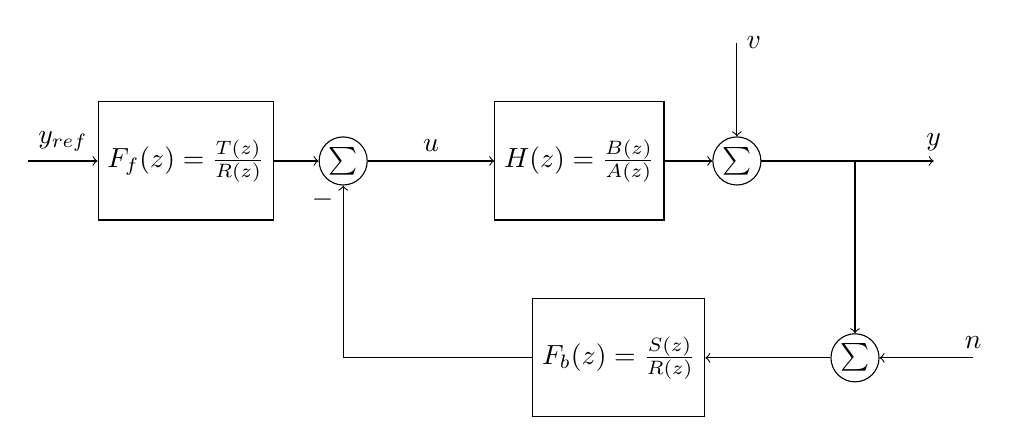
\begin{tikzpicture}[
    node distance=2cm, block/.style={rectangle, draw, minimum height=15mm, minimum width=20mm}, sumnode/.style={circle, draw, inner sep=1pt}]

  \node[coordinate] (input) {};
  \node[block, right of=input] (TR) {$F_f(z)=\frac{T(z)}{R(z)}$};
  \node[sumnode, right of=TR] (sum) {$\sum$};
  %\node[block,right of=sum, node distance=30mm] (plant) {$H(z)=\frac{B(z)}{A(z)}$};
  \node[block,right of=sum, node distance=30mm] (plant) {$H(z)=\frac{B(z)}{A(z)}$};
  \node[sumnode, right of=plant] (sumdist) {$\sum$};
  \node[coordinate, above of=sumdist, node distance=15mm] (dist) {};
  \node[coordinate, right of=sumdist, node distance=15mm] (measure) {};
  \node[coordinate, right of=measure, node distance=10mm] (output) {};
  \node[sumnode,below of=measure, node distance=25mm] (sumnoise) {$\sum$};
  \node[coordinate, right of=sumnoise, node distance=15mm] (noise) {};
  %\node[block,left of=sumnoise, node distance=20mm] (delay) {$\frac{1}{z^2}$};
  \node[block,left of=sumnoise, node distance=30mm] (SR) {$F_b(z) = \frac{S(z)}{R(z)}$};

  \draw[->] (input) -- node[above] {$y_{ref}$} (TR);
  \draw[->] (TR) -- node[above] {} (sum);
  \draw[->] (sum) -- node[above] {$u$} (plant);
  \draw[->] (plant) -- (sumdist);
  \draw[->] (dist) -- node[at start, right] {$v$} (sumdist);
  \draw[->] (sumdist) -- node[at end, above] {$y$} (output);
  \draw[->] (measure) -- (sumnoise);
  \draw[->] (noise) -- node[at start, above] {$n$} (sumnoise);
  \draw[->] (sumnoise) -- (SR);
  %\draw[->] (delay) -- (SR);
  \draw[->] (SR) -| (sum) node[left, pos=0.96] {$-$};
\end{tikzpicture}
\end{center}

We desire a closed-loop system from the reference signal \(y_{ref}\) to the output \(y\)  with pulse-transfer function
\[H_c(z) = \frac{0.1643(z+1)}{z^2 - 1.637z + 0.6703} \]
The S- and R- polynomials have been found from the Diophantine equation
\[ A(z)R(z) + B(z)S(z) = (z^2 - 1.637z + 0.6703)(z - 0.67)\]
to be
\begin{equation*}
\begin{aligned}
  R(z) &= z - 0.368\\
  S(z) &= 4.98z - 4.076
\end{aligned}
\end{equation*}

Determine the feedforward  (prefilter) part of the controller \(F_f(z) = \frac{T(z)}{R(z)}\) so that the desired closed-loop pulse-transfer function is obtained.

%\end{document}

\section*{Solutions}

\subsection*{Problem 1}
\subsubsection*{(a)}
With the small-angle approximations we get the system of first-order differential equations
\begin{equation*}
\begin{aligned}
\frac{d}{dt}  \bbm \theta\\\dot{\theta} \ebm &= \bbm \dot{\theta}\\ \frac{mgl}{J}\theta + \frac{1}{J}u \ebm, \qquad y = \theta
\end{aligned}
\end{equation*}
which written on matrix-vector form is 
\begin{equation*}
\begin{aligned}
\frac{d}{dt}  \bbm \theta\\\dot{\theta} \ebm &= \bbm 0 & 1\\ \frac{mgl}{J} & 0\ebm \bbm \theta\\\dot{\theta} \ebm + \bbm 0\\\frac{1}{J} \ebm u\\
y &= \bbm 1 & 0 \ebm \bbm \theta\\\dot{\theta} \ebm.
\end{aligned}
\end{equation*}

\subsubsection*{(b)}
The expression 
\begin{equation*}
G(s) = C \big( sI- A\big)^{-1} B
\end{equation*}
for how to go from a state-space model to a transfer function is obtained by taking the Laplace-transform of the state-space model (this part is not needed to show). Note that 
\[ (sI-A)^{-1} = \bbm s & -1\\-\frac{mgl}{J} & s\ebm^{-1} = \frac{1}{s^2 - \frac{mgl}{J}} \bbm s & 1\\\frac{mgl}{J} & s\ebm. \]
Inserting into the expression we get
\begin{equation*}
\begin{aligned}
G(s) = C \big( sI- A\big)^{-1} B = \frac{1}{s^2 - \frac{mgl}{J}}  \bbm 1 & 0 \ebm \bbm s & 1\\\frac{mgl}{J} & s\ebm \bbm 0\\\frac{1}{J}\ebm = \frac{ 1/J }{s^2 - \frac{mgl}{J}}.
\end{aligned}
\end{equation*}
The poles are the roots of the characteristic polynomial \(s^2 - \frac{mgl}{J}\), which clearly are
\(\pm \omega_0\) where \(\omega_0 = \sqrt{\frac{mgl}{J}}\).


\subsubsection*{(c)}

The discrete-time state-space model is given by
\begin{equation*}
\begin{aligned}
  x(kh+h) &= \Phi(h) x(kh+h) + \Gamma(h) u(kh)\\
  y(kh) &= C x(kh),
\end{aligned}
\end{equation*}
where 
\[ \Phi(h) = \mexp{Ah}, \qquad \Gamma(h) = \int_0^h \mexp{A\tau} d\tau.\]

We get
\begin{equation*}
\begin{aligned}
  \Phi(h) &= \mexp{Ah} = \Lap^{-1} \{ (sI-A)^{-1}\} =  \Lap^{-1} \{ \bbm s & -1\\ -\omega_0^2 & s\ebm^{-1} \}\\
  &= \Lap^{-1} \{ \frac{1}{s^2 - \omega_0^2} \bbm s & 1\\\omega_0^2 & s\ebm \}
   = \bbm \Lap^{-1} \frac{s}{s^2 - \omega_0^2} & \frac{1}{s^2 - \omega_0^2}\\\frac{\omega_0^2}{s^2 - \omega_0^2} & \frac{s}{s^2 - \omega_0^2}\ebm\\
   &= \bbm \cosh(\omega_0 h) & \frac{1}{\omega_0} \sinh(\omega_0 h)\\\omega_0 \sinh(\omega_0 h) & \cosh(\omega_0 h) \ebm.
 \end{aligned}
\end{equation*}
\begin{equation*}
\begin{aligned}
  \Gamma(h) &= \int_0^h \mexp{A\tau} d\tau = \int_0^h \bbm \frac{1}{\omega_0} \sinh(\omega\tau)\\ \cosh(\omega_0 \tau) \ebm d\tau
  = \bbm  \frac{1}{\omega_0^2} \cosh(\omega_0\tau) \Big|_0^h\\[3mm]  \frac{1}{\omega_0}\sinh(\omega_0\tau) \Big|_0^h\ebm \\
  &= \bbm \frac{1}{\omega_0^2}\big( \cosh(\omega_0 h) - 1 \big)\\ \frac{1}{\omega_0} \sinh(\omega_0h) \ebm. 
\end{aligned}
\end{equation*}

\subsection*{Problem 2}

\begin{enumerate}
\item The sampling period should be related to the speed of the closed-loop system, since we have given the desired closed-loop poles. In continuous-time this is a second order critically-damped system with double-pole in $s=-\omega_0=-1$. The step-response of such a system is given by \[ y(t) = 1 - (1+t)\mexp{-t}\]
  \begin{center}
    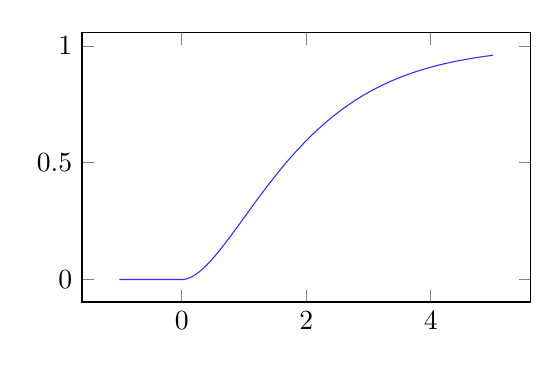
\begin{tikzpicture}
      \begin{axis}[
        width=0.6\linewidth,
        height = 5cm,
        ]
        \addplot+[no marks, blue!80, domain=-1:5, samples=400] { (x>0)*(1 - exp(-x)*(1+x))};
      \end{axis}
    \end{tikzpicture}
  \end{center}
  The rise-time is about 4 seconds, and using the rule-of-thumb that the number of sampling perdiods should be 4-10, we may for instance choose $h=0.5$. This gives the state-space model
  \begin{equation*}
    \begin{aligned}
      x(k+1) &= \bbm 1.13 & 0.52\\0.52 & 1.13 \ebm x(k) + \bbm 0.13\\0.52 \ebm u(k)\\
      y(k) &= \bbm 1 & 0 \ebm x(k).
    \end{aligned}
  \end{equation*}
\item Calculate the state feedback gain $L$ in 
  \[ u(kh) = -l_1 x(kh) - l_2 x(kh) = -L x(kh)\]
  so that the closed loop systems has the desired poles. With the negative state feedback we get a closed-loop system with characteristic polynomial given by 
  \begin{equation*}
    \begin{aligned}
      \det \big(zI - (\Phi - \Gamma L)\big) &= \det \left( \bbm z & 0\\ 0 & z\ebm - \left(\bbm 1.13 & 0.52\\0.52 & 1.13 \ebm - \bbm 0.13 l_1 & 0.13 l_2\\ 0.52 l_1 & 0.52 l_2 \ebm\right)\right)\\
      &= \det \bbm z-1.13+0.13l_1 & -0.52+0.13l_2\\ -0.52 + 0.52l_1 & z-1.13+0.52l_2 \ebm\\
      &= (z-1.13+0.13l_1)(z-1.13+0.52l_2) - (-0.52 + 0.52l_1)(-0.52+0.13l_2)\\
      &= z^2 + (0.13l_1 + 0.52l_2 - 2.26)z + 0.1235l_1 - 0.52l_2 + 1.0065.
    \end{aligned}
  \end{equation*}
  Setting each coefficient equal to those of the desired characteristic polynomial \((z-\mexp{-0.5})^2 = (z-0.607)^2 = z^2 - 1.21z + 0.368\) gives the system of equations
  \begin{equation*}
    \begin{aligned}
      \bbm 0.13 & 0.52\\0.1235 & -0.52 \ebm \bbm l_1\\l_2 \ebm = \bbm -1.21 + 2.26\\0.368-1.0065 \ebm
    \end{aligned}
  \end{equation*}
  with solution
  \[ l1 =  1.61 \qquad l2= 1.61 \]
\item Verify your calculations using matlab. 
  \begin{verbatim}
omega0 = 1;
h = 0.5;
Phi = [cosh(omega0*h), 1/omega0*sinh(omega0*h)
    omega0*sinh(omega0*h), cosh(omega0*h)]
Gamma = [1/omega0^2*(cosh(omega0*h) - 1); 1/omega0*sinh(omega0*h)]
L = [1.61, 1.61];
eig(Phi-Gamma*L)

ans =

   0.606530659712637
   0.604280024872918
\end{verbatim}
\item The observer poles should be at least twice as fast as the closed-loop poles. Twice as fast means two poles in \(z = \mexp{-2\omega_0 h} = \mexp{-1} \approx 0.368\). 
\end{enumerate}

\subsection*{Problem 3}

We only need to determine the polynomial \(T(z)\). The closed-loop transfer function from the reference signal to the output is, according to the block-diagram and using Mason's rule
\begin{equation*}
  \begin{aligned}
    H_c(z) &= \frac{ \frac{T}{R} \frac{B}{A} }{1 + \frac{S}{R} \frac{B}{A}} = \frac{ TB}{AR + BS} = \frac{T(z)B(z)}{A_{cl}(z)}\\
    &= \frac{T(z)0.02(z+1)}{(z^2 - 1.637z + 0.6703)(z-0.67)},
  \end{aligned}
\end{equation*}
which should be equal to the desired closed-loop transfer function
\[H_c(z) = \frac{0.1643(z+1)}{z^2 - 1.637z + 0.6703}. \]
This gives
\[ \frac{T(z)0.02(z+1)}{(z^2 - 1.637z + 0.6703)(z-0.67)} = \frac{0.1643(z+1)}{z^2 - 1.637z + 0.6703}. \]
Solving for \(T(z)\) gives
\[ T(z) = \frac{0.1643}{0.02}(z-0.67).\]

You would arrive at the same result if you identified \((z-0.67)\) as the observer polynomial, and followed the usual route of setting \(T(z) = t_0A_o(z)\) and solving for \(t_0\) so that the closed-loop system have unit static gain.


\end{document}
